\documentclass[a4paper,12pt]{report}
\usepackage{titlesec}
\usepackage{graphicx}
\usepackage{fancyhdr}
\usepackage{geometry}
\usepackage{indentfirst}
\usepackage{plantuml}
\usepackage{tikz}
\usepackage{aeguill}
\usepackage{float}

% chktex-file 44

\newgeometry{
    top=2.5cm,
    bottom=3cm,
    inner=2cm,
    outer=2cm,
}

\pagestyle{fancy}
\fancypagestyle{plain}{}

\lhead{\scriptsize Computing and Information Technology\\
    2022\\
    David Daniel, Pava\\
    Walman: A Virtual Wallet Management System}
\rhead{
\includegraphics[width=4cm]{images/logo_upt.jpg}}
\cfoot{- \thepage\ -}
\renewcommand{\headrulewidth}{0pt}

\setlength{\headheight}{44pt}

\fancypagestyle{titlepage}{
    \lhead{\footnotesize Computing and Information Technology\\\textbf{2022}}
    \rhead{
\includegraphics[width=4cm]{images/logo_upt.jpg}}
    \cfoot{}
}

\titleformat{\chapter}{\center\normalfont\LARGE\bfseries\MakeUppercase}{\thechapter}{0.5em}{}
\titlespacing*{\chapter}{0pt}{3.5ex plus 1ex minus .2ex}{2.3ex plus .2ex}
\title{\LARGE WALMAN\\{ A Virtual Wallet Management System}}

\titleformat{\section}{\normalfont\large\bfseries\MakeUppercase}{\thesection}{0.5em}{}
\titlespacing*{\chapter}{0pt}{3.5ex plus 1ex minus .2ex}{2.3ex plus .2ex}
\title{\LARGE WALMAN\\{ A Virtual Wallet Management System}}

\author{Candidate: David Daniel, Pava
    \\Coordinator: Assoc. Prof.\ Razvan, Bogdan}

\date{June 2022 Session}

\begin{document}

\begin{titlepage}
    \thispagestyle{titlepage}
    \begin{center}
        \vspace*{10cm}
        \LARGE\textbf{Walman\\A Virtual Wallet Management System}\\
        \vfill
    \end{center}
    \begin{flushleft}
        \large\textbf{Candidate: David Daniel, Pava
            \\Coordinator: Assoc. Prof.\ Razvan, Bogdan}
    \end{flushleft}

\end{titlepage}

\chapter*{Abstract}

\tableofcontents

\chapter{Introduction}
In this project I implemented a wallet manager in the form of a mobile
application. The main features are password management, password generation, qr
and barcode storage and management, crypto wallet and OTP token management. The
user has the option to backup the data either in the cloud or on the
blockchain. Once backed up, the data will be available to be restored.

\section{Context}

\par In the last 30 years, the number of tasks that are digitalized has increased
exponentially. The most important part of the security systems of these tasks
is user management and authentication. The password is the most widely spread
form of user authentication and thus is often the prime target of attackers
that want to impersonate someone else.

According to~\cite{systematicAnalysis}, a \textit{``systematic literature
    review in the area of passwords and passwords security''}, there are many
problems with password security and management ranging from weak passwords and
password reuse, to users writing down passwords or sending them through
unsecure channels. Most of these problems according
to~\cite{systematicAnalysis} are solved by using password recommendations. A
good solution to most of these problems is a password management tool. A
password manager is a piece of software designed for generating and managing
passwords, in this way the user can have unique, complex and safely stored
password without having to remember them.

Another great method to better secure you accounts is using a two factor
authentication (2FA) method. These method vary from security questions, to one
time passwords (OTP) sent from the server to the user via email or SMS, to OTPs
generated using specialized algorithms such as: HMAC-based One Time Password
(HOTP)\cite{hotp} and Time Based One Time Password (TOTP)\cite{totp}.

The cryptocurrency market is another area that has seen a considerable
development lately. As of May 2022, the market cap of Bitcoin is around 565
billion USD, and the market cap of Ethereum is around 214 billion USD.\@ In the
case of Bitcoin, that is more than double of what it was in 2019 (around 211
billion USD), referenced in~\cite{cryptocurrencyMarketAnalysis}.
Cryptocurrencies also offer secure and long term storage capabilities thanks to
the blockchain technology. Blockchain backups, thanks to the decentralized
nature of the blockchain, are very hard to be tempered with. A traditional
cloud backup could be lost or inaccessible in more than one situations. The
most obvious one is data loss happening as result of a cyber attack or the
company simply going bankrupt. There are also situations in which the company
itself can refuse to serve you anymore. They can freeze your account or just
refuse to serve an entire country all-together, we have the recent example of
companies like Visa and Mastercard refusing to serve russian citizens as result
of political tensions. All these scenarios cannot happen in a decentralized
blockchain system.

Businesses that were traditionally not online like shopping also have inversely
digitalized. Nowadays most of the hypermarkets offer fidelity cards. Usually
these cards are built around a unique barcode or qr code. Often it's hard to
manage all your cards, so a digital storage solution to solve this issue would
help the end user better manage their cards.

Considered all mentioned above, a user has to remember and manage a lot of
information in order to interact with the currently available online
infrastructure. A tool that could help them manage all this data better is a
wallet manager.

\section{Motivation}

My personal motivation for creating a wallet manager is the fact that I want to
use it myself. Also I wanted for a long time to explore the state of the art in
smart contract development, so this was a great occasion to do so.

I chose to create this project in the form of a mobile application since people
tend to have their smartphones with them most of the time, so having a virtual
wallet on your mobile device makes sense.

Another factor that motivates me is the fact that currently in the mobile
application market there are almost no free and open source password management
applications available. The user needs to \textit{trust} the creators of the
application with their data, not knowing how the implementation of the product
is made, they have no guarantee that the data is safe.

\section{Similar Products Available on the Market}

There are a lot of password managers available on the market. In this section
we are going to try to make a comparison between some of the most popular
options available.

\begin{table}[h!]
    \centering
    \begin{tabular}{ | l | l | l | l | l | l | }
        \hline
        \textbf{Property}           & \textbf{LastPass} & \textbf{RememBear} & \textbf{KeePass} & \textbf{PassMan} & \textbf{KeyBase} \\
        \hline
        \textbf{Mobile Version}     & Yes               & Yes                & No               & Yes              & Yes              \\
        \hline
        \textbf{Blockchain Storage} & No                & No                 & No               & No               & Yes              \\
        \hline
        \textbf{Price}              & \$3/month         & \$6/month          & Free             & Free             & Free             \\
        \hline
        \textbf{License}            & Proprietary       & Proprietary        & GPL-2.0          & AGPL-3.0         & BSD-3            \\
        \hline
    \end{tabular}
    \caption{A comparison between some of the most popular password managers.}\label{tab:otherProducts}
\end{table}

First off we have LastPass\cite{lastpass} and RememBear\cite{remembear}, two
very similar password managers, both having a free and a payed plan. Neither of
these two is open source, so the most pressing issue regarding them is the
guarantee that your data is safe. Without having the ability to see how your
data is managed and stored you cannot be certain that it is secure. Also these
applications do not have blockchain backups.

KeePass\cite{keepass} is probably the most popular password manager for
desktop. It is free and open source, and the code was analyzed and certified by
specialized organizations such as the Open Source Initiative. The biggest
drawback to KeePass is the aged user interface and the missing mobile
application counterpart. Nowadays a lot of the situations where a user needs
access to their credentials are happening while using smartphones. Also the
features are limited, KeePass doing one thing and doing it well that being
password management. There are no cloud or blockchain backups, so the user
needs to manager backing up and storing their password database themselves.

Similar with KeePass, PassMan\cite{passman} is a free and open source password
manager. They have a mobile version of the application, but blockchain backups
are missing. Also, again, PassMan is just a password manager. It does not
manage shopping cards or crypto wallets.

Last but not least there is KeyBase\cite{keybase} which is not technically a
password manager. KeyBase is a blockchain, decentralized, social media
application. You can store password and secure notes inside the application but
from the user experience point of view, KeyBase was never designed to be a
password or wallet manager. The reason why it is mentioned, is because KeyBase
is implemented on the blockchain, all user data is encrypted and it's free and
open source.

\chapter{Technology Stack}

In this chapter I am going to describe the technologies used. The application
has 3 main components. The first component is the frontend, a mobile
application. The second one is the cloud storage backend. The last part are the
smart contracts deployed on the blockchain.

\section{Frontend}

The most important aspects I considered when I chose the technologies used for
the frontend was cross-platform capabilities, ease of testing, documentation
availability and performance. This is why for this project I chose a Flutter
stack.

\subsection{Flutter}

Flutter\cite{flutterDocs} is a mobile application development framework
developed by Google in the Dart programming language. It was released in May
2017 and it currently is one of the most popular mobile development frameworks.

According to \textit{``An empirical investigation of performance overhead in
    cross-platform mobile development frameworks''}\cite{flutterPerformance},
Flutter has one of the better resource management systems when compared with
other popular mobile development frameworks.

\begin{figure}[H]
    \centering
    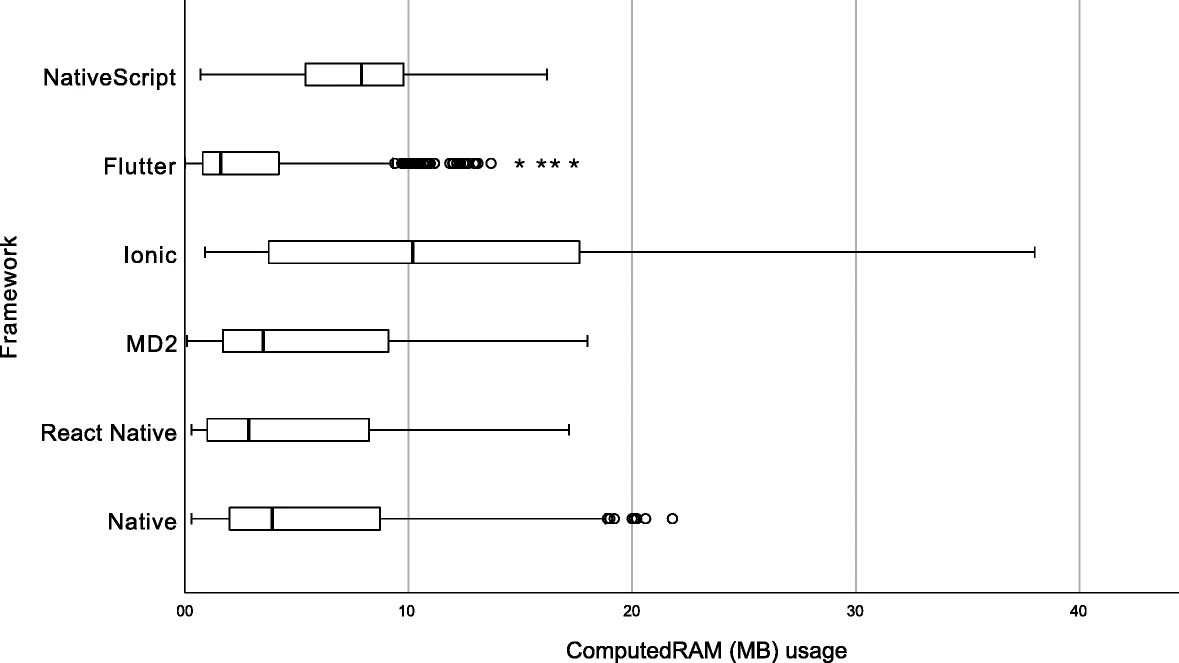
\includegraphics[scale=0.4]{images/flutterPerformance/ram.png}
    \caption{Boxplot from~\cite{flutterPerformance} of RAM usage across all tests done in~\cite{flutterPerformance} }\label{fig:flutterPerformanceRAM}
\end{figure}

As seen in~\ref{fig:flutterPerformanceRAM}, on average Flutter outperforms most
of the other frameworks in memory management.

\begin{figure}[H]
    \centering
    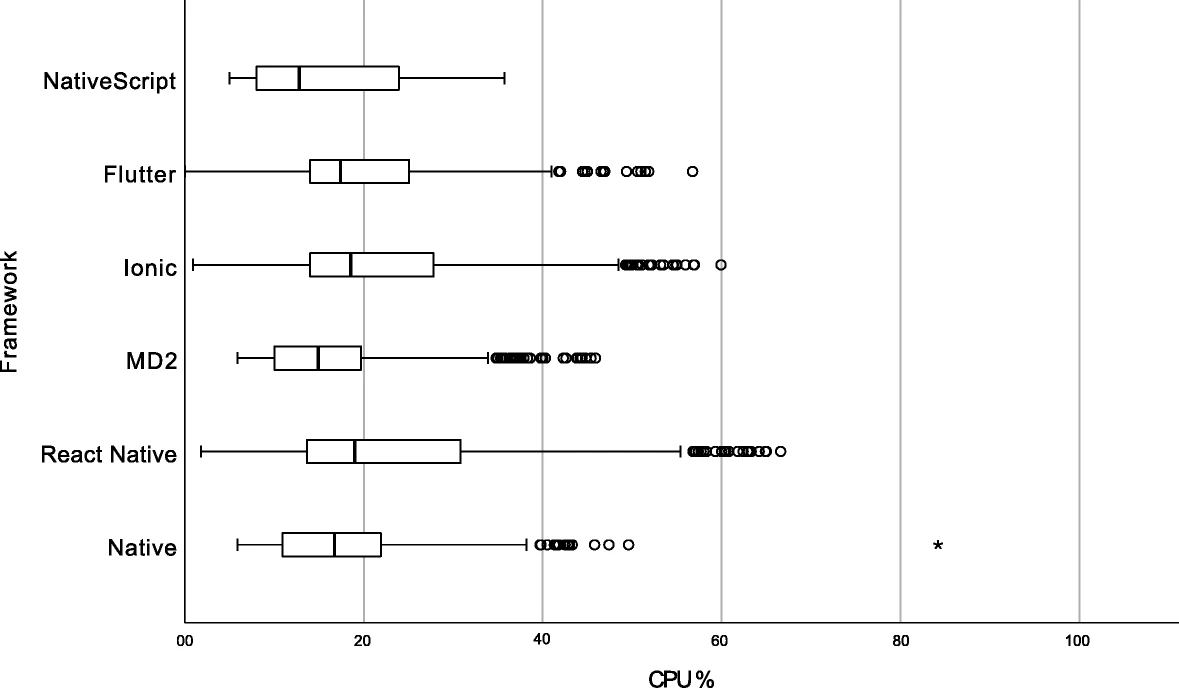
\includegraphics[scale=0.4]{images/flutterPerformance/cpu.png}
    \caption{Boxplot from~\cite{flutterPerformance} of CPU usage across all tests done in~\cite{flutterPerformance} }\label{fig:flutterPerformanceCPU}
\end{figure}

In~\ref{fig:flutterPerformanceCPU} we have a comparison between CPU usage of
similar applications implemented in different frameworks
in~\cite{flutterPerformance}, where Flutter achieves a competitive result when
compared to the other frameworks.

Another very important feature of Flutter is cross-platform compatibility. A
mobile application developed in this framework can be build in native Android
and IOS applications with minimal performance loss. There is also Flutter Web
for web applications, offering the option to create a browser variant of the
application in the future, reusing already developed and tested parts from the
mobile application.

Flutter comes with a very rich and detailed documentations, the Flutter
Docs\cite{flutterDocs} and a set of development plugins for the most used IDE
and text editors such as Android Studio, Intellij or Visual Studio Code. During
the development process the code is executed into a runtime environment,
allowing almost instant compilation times speeding up the development, and in
production, the code is compiled into a native application for performance
enhancement.

The User Interface in Flutter is build based on a widget tree, similar to
React. Every User Interface item inherits the Widget class.

\subsection{Dart}\label{chapter:dart}

Dart\cite{dartDocs} is a general purpose programming language developed by
Google starting with 2011. It was intended to replace JavaScript and TypeScript
for frontend applications, but instead, later, it was used to create the
Flutter framework.

Dart is a type safe, C-like programming language. It can be both interpreted by
a runtime or compiled. The memory management is handled by a garbage collector
similar with Python or JavaScript.

One of the strongest features of Dart is the compiler. It can be compiled in
binary code, JavaScript or mobile native code such as Java and Kotlin for
Android and Objective-C and Swift for IOS devices. Dart also performs tree
shaking at compile time, discarding unused objects, methods and functions.

\subsection{Code Generation}

During the development of the project I used multiple packages (dart libraries)
in the process. One very important package that needs to be mentioned is the
\textit{freezed} package\cite{freezedDocs}. This offers code generation for
common model functionalities such as json encoders and decoders, copyWith
methods, different constructors and access functions and more.

Classes generated by the package are annotated with the \textit{@freezed} tag.
The generated code is stored into files that contain the \textit{.freezed.dart}
and \textit{.g.dart} extensions.

\subsection{State Management}

One of the most important aspects of frontend application development is state
management architecture. There are a lot of different state management patterns
available in Flutter\cite{flutterStateManagement} such as Provider, BLoC or the
simple setState. These state management patterns tell the application when the
state has changed and when certain components of the presentation layer (the UI
of the application) needs to be updated as a result of that.

For this project I used the Redux state management architecture. This pattern
is a very popular solution for managing the state of an application, and it is
commonly used in web development. There is an implementation for it in Flutter
in the packages: flutter\_redux\cite{flutterReduxDocs}, redux\cite{reduxDocs}
and redux\_epics\cite{reduxEpicsDocs}.

\begin{figure}[H]
    \centering
    \scalebox{0.75}{\input{diagrams/component/redux.latex}}
    \caption{Basic structure of a Redux State Management System}\label{fig:reduxArchitecture}
\end{figure}

In~\ref{fig:reduxArchitecture} we can see the core structure of the redux
architecture I used in the project. A state change begins the dispatch of an
action. They are usually triggered by the user interface, but in some cases
they can be triggered by an API event. The Epics are a set of listeners which
analyze the action stream. When an Epic recognizes an Action, it performs a
series of operations which can process the data using the APIs (business logic)
or dispatch new actions. Every action is also watched by the Reducer, which
listens for Actions and changes the State accordingly. When the State changes,
the Widgets (in case of Flutter) that depend on the elements updated in the
State, are triggered to pe updated.

In order to access specific elements of the state, and not update every widget,
every time the state changes. Containers can be used to access a specific part
of the state. In order to access the State, the User Interface needs to request
it from the Store, in this way, the Store knows when to redraw the object. The
widgets that update when the state is modified and have access to the Store are
part of the flutter\_redux package\cite{flutterReduxDocs}.

Error handling in redux is made using special stream functions from the RxDart
package\cite{rxDart}. RxDart offers and extension to the functional
capabilities of dart. In redux the application is represented as a stream of
actions. In order to make error handling efficiently, every action sequence
spawns a new stream. In case of an exception, the stream will have an exception
and we can dispatch a new Action with relevant information about the error. In
this way the probability of total application wide runtime exceptions is
dramatically lowered.

\section{Firebase}

\subsection{User Management}

\subsection{Firestore}

\section{Blockchain}

\subsection{Ethereum}

\subsection{Smart Contracts}

\subsection{Solidity}

\subsection{Test Networks}

\section{Development Environment}

\chapter{Implementation}

\section{Use Cases}

\section{System Architecture}

\section{Password Management}

\section{QR and Barcode Management}

\section{OTP Authenticator}

\subsection{HOTP}

\subsection{TOTP}

\section{Cryptocurrency Wallet}

\section{Backup}

\subsection{Cloud Backup}

\subsection{Blockchain Backup}

\section{Security}

\chapter{Tests}

\section{Test Pipeline}

\section{Unit Tests}

\section{Widget Tests}

\section{Performance Statistics}

\chapter{Conclusions}

\section{Possible Improvements}

\bibliographystyle{plain}
\bibliography{references}
\addcontentsline{toc}{chapter}{Bibliography}

\end{document}